\section{Framework Overview}\label{sec-arch}
The basic structure of SVC is: (1) analyze a view maintenance procedure to efficiently compute an up-to-date sample, (2) use this sample to correct stale query results, and (3) use an index of outliers make the sample robust to outliers in the data. 
The key insight is that SVC reduces the cost of view maintenance making it feasible to apply in resource-constrained settings where frequent maintenance was once impossible.
We first define notation, terminology, and the problem setting that we address in this work.
Then, we formalize the three problems that the different components of SVC address: (1) analyzing a maintenance procedure to efficiently maintain a sample, (2) query processing using the sample, and (3) using an outlier index.
Finally, we overview the system architecture and discuss a toy numerical example of how this works in practice.

\subsection{Notation}
%\reminder{You have defined $\mathcal{D}$, $\{R_i\}$, etc in Definition 1. Maybe you can move Def 1 to this Section?}
Let $\mathcal{D}$ be a database which is a collection of relations $\{R_i\}$, and let $S$ be a materialized view of this database.
We denote the set of insertions to a relation $R_i$ as $\Delta R_i$ and deletions as $\nabla R_i$.
In this paper, we refer to $\Delta R_i$ and $\nabla R_i$ as ``delta relations".
An update to a relation can be modeled as a deletion and then an insertion.

When the base relations have been updated (there exists insertions and/or deletions), queries on the view $S$ will be stale.
We call the procedure to update the view as a \emph{maintenance strategy} $\mathcal{M}$.
A maintenance strategy is a relational expression the execution of which will update the view $S$, and we call the updated view $S'$.

\begin{definition}[Maintenance Strategy]
Let, $\mathcal{D}$ be a database which is a collection of relations $\{R_i\}$.
Let, $S$ be a materialized view.
We denote the insertions to a relation $R_i$ as $\Delta R_i$ and the deletions as $\nabla R_i$.
A maintenance strategy $\mathcal{M}$ is a relational expression the execution of which updates the view.
It is a function of the database $\mathcal{D}$, $S$, and all the delta relations $\{\Delta R_i\} \cup \{\nabla R_i\}$.
\end{definition}

%In this work, we ignore \textbf{null} types and assume that each tuple in the relation has non-null attribute values.
We look at maintenance strategies composed of the following relational operations:
\begin{itemize}\vspace{-.45em}
\item $\sigma_{\phi}(R)$: Selection select all tuples $r$ from $R$ that satisfy the restriction $\phi (r)$ \vspace{-.45em}
\item $\Pi_{a_1,a_2,...,a_k}(R)$: Projection select attributes $\{a_1,a_2,...,a_k\}$ from R \vspace{-.45em}
\item $\bowtie_{\phi (r1,r2)}(R_1,R_2)$: Join select all tuples in $R_1 \times R_2$ that satisfy $\phi (r_1,r_2)$.
\item $\gamma_{f,A}(R)$: Apply the aggregate function $f$ to the relation R grouped by the distinct values of $A$, where $A$ is a subset of the attributes. The output schema is of the result is $a, f_i$. \footnote{A special case of this operator is $\delta$ the deduplication operator i.e. $f$ always returns null. Another special case, is when there is a expression in the group by clause which we treat as creating a set of virtual columns.}\vspace{-.45em} 
\item $R_1 \cup R_2$: Set union take a union of the two sets.
\item $R_1 \cap R_2$: Set intersection take an intersection of the set.
\item $R_1 - R_2$: Set difference.
\end{itemize}
Relational expressions can be expressed in a tree form which we call an \emph{expression tree}.

To illustrate the concept of a maintenance strategy, consider the following view that finds view counts for all videos:
\begin{lstlisting} 
CREATE VIEW countView
AS SELECT 
	videoId,
	count(1) AS visitCount,
FROM 
	Log, Video
WHERE 
	Log.videoID = 
		Video.videoID
GROUP BY 
	videoId;
\end{lstlisting}
If new records have been added to \tbl{Log} and \tbl{Video}, then the maintenance strategy consists of the following expressions: (1) create a ``delta view" by applying the view definition to \tbl{LogIns}, (2) update the view by taking the join of the ``delta view" with \tbl{countView}, (3) project the result by incrementing \tbl{visitCount}. We illustrate this process with the expression tree in Figure \ref{exexpr}.

\begin{figure}[t] \vspace{-2em}
\centering
 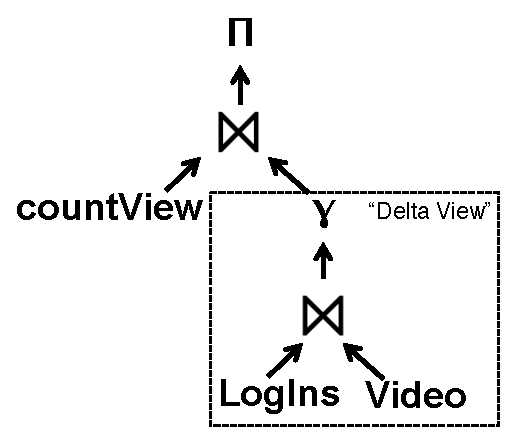
\includegraphics[scale=0.50]{figs/example_expression_tree.pdf} \vspace{-.25em}
 \caption{For our example, we represent the expression tree of the maintenance strategy. We first calculate a delta view using the new insertions and then join this view with the old view.\label{exexpr}}\vspace{-1.75em}
\end{figure}

\subsection{Sampling}
In this work, we focus on uniform samples of views.
We define a sampling ratio $m\in [0,1]$ and for each row in a view $S$, we include it into a sample with probability $m$.
To differentiate sampled relations from un-sampled ones we use the ``hat" notation eg. $\hat{S}$. 

While, uniform sampling supports a wide variety of query types, it may have issues with queries with highly selective predicates.
In principle, our framework can be extended to handle stratified samples similar to the BlinkDB project \cite{AgarwalMPMMS13}.
However, this requires that we know our query workload in advance.  
In this paper, we do not discuss stratified sampling and will explore this further in future work.

Note, that this definition is slightly different from the reservoir sampling techniques studied in AQP \cite{DBLP:journals/toms/Vitter85} which find a uniform sample of fixed \emph{size} $k\le \mid S \mid$.
Our sampling ratio gives a sample of the size $k$ in expectation, however, the actual size from any given instance may be slightly different.
For large sample sizes, there is little difference between the techniques since the actual size of using a sample ratio will be close to $k$.
The uniform sample model represents our algorithm which uses hashing better and also makes the presentation of our analysis more clear.

Furthermore, any ``black-box" uniform sampling algorithm can be used to achieve a reservoir sample.
The use of one technique over another does not affect the general principles or the statistics of SVC, only the 
notation in the analysis.

\subsection{Problem Statements}
\subsubsection{View Maintenance as Data Cleaning}
In SVC, we model staleness in a materialized view as a type of data error.
Materialized views whose base relations have been updated potentially give stale query results.
We formalize the problem of correcting staleness as a data cleaning operation.

If we are given a materialized view $S$ and we know the base relations have had insertions and deletions, then there are three possible types of error:
\begin{itemize}
\item A row in $S$ needs to be updated.
\item A row in $S$ needs to be deleted.
\item A new row needs to be inserted into $S$.
\end{itemize}

In this case, it is clear that simply executing the maintenance strategy $\mathcal{M}$ will achieve the necessary results and update the view $S$ to view $S'$.
However, now suppose we have a sampled view $\hat{S}$, and we want to do just enough effort to update only the rows in the sample.
This problem is challenging since the errors are not just updates to rows in the views, as there might be new insertions needed.
Thus, we define cleaning in the following way: suppose we have a stale uniform sample $\hat{S}$ with sampling ratio $m$, we want to find an up-to-date uniform sample $\hat{S'}$.
We define the cleaning procedure as preserving the uniformity of sampling, so after cleaning $\hat{S'}$ is a uniform sample of $S'$:
\begin{itemize}
\item If an update is needed, update the row.
\item If the row needs to be deleted, delete the row.
\item For all new rows that need to be inserted into the view $S'$ insert a random sample of ratio $m$.
\end{itemize}
It is important to note that the way we defined data cleaning on a sample does not necessarily give a unique $\hat{S'}$. 
In this paper, we take advantage of this property and propose a technique that analyzes $\mathcal{M}$ and can find a particular $\hat{S'}$
efficiently.

In, SampleClean \cite{wang1999sample}, \nsc query result estimation is done taking a row-by-row difference of the dirty and cleaned data.
However, in prior work, we did not consider the effect of deletions or insertions so taking this difference was well defined.
In this application, we have to define a new property to handle this problem, which we call ``correspondence".
SVC compares two ``corresponding" samples to derive a correction. 
\begin{definition}[Correspondence]
$\hat{S'}$ and $\hat{S}$ are uniform samples of $S'$ and $S$, respectively.  We say $\hat{S'}$ and $\hat{S}$ correspond if and only if:
\item For every row $r$ in $\hat{S}$ that required a delete, $r \not\in \hat{S'}$
\item For every row $r$ in $\hat{S}$ that required an update, $r\in \hat{S'}$
\item For every row $r$ in $\hat{S}$  that was unchanged, $r \in \hat{S'}$
\item For every row $r$ in $S$ but not in $\hat{S}$, $r \not\in \hat{S'}$
%\item For every row $r$ in $S'$ that is newly inserted, $r \not\in \hat{S}$.
%\item If a row $r$ requires an update and then a deletion. The deletion takes precedence and $r \not\in \hat{S'}$.
%\item Rows that are inserted trivially satisfy the conditions since those rows are not contained in $S$ or $\hat{S}$.
\label{correspondence}
\end{definition}
This definition of correspondence gives us a way to get two samples from which we can take a row-by-row difference.
There is some nuance in how to handle null values which we discuss in Section \ref{correction}.

\begin{example}[Correspondence]
Suppose \tbl{countView} has 4 videos: 
\begin{lstlisting} [mathescape]
V1 (visitCount = 4), V2 (visitCount = 6), V3 (visitCount = 1), V4 (visitCount = 1)
\end{lstlisting}
We take a sample of \tbl{countView} and call it \tbl{countViewSample} that contains V1 and V2.
\tbl{LogIns} has new logs of 1 visit for V1 and 1 visit for a new video V5.
An up-to-date sample that corresponds is:
\begin{lstlisting} [mathescape]
V1 (visitCount = 4+1), V2 (visitCount = 6)
\end{lstlisting}
An up-to-date sample that does \emph{not} corresponds is: 
\begin{lstlisting} [mathescape]
V1 (visitCount = 4+1), V3 (visitCount = 1)
\end{lstlisting}
This is because V2 was unchanged and therefore should be included in the sample.
\end{example}

\subsubsection{Query Correction}
Given a query $q$ which has been applied to the stale view $q(S)$ giving a stale result.
Our query correction component takes two corresponding samples $\hat{S'}$ and $\hat{S}$, and calculates a correction to $q(S)$.
Like similar restrictions in other sampled-based systems \cite{agarwalknowing}, there are restrictions on the queries $q$ on the view that we can answer. 
In the SampleClean work, we focused on \sumfunc,\countfunc, and \avgfunc queries of the form: 
\begin{lstlisting} [mathescape]
SELECT $f(a)$ FROM View 
WHERE Condition(A);
\end{lstlisting}
In this work, we expand the scope of the query processing, and consider general non-nested aggregate queries with simple predicates.

We also consider correcting stale non-nested select queries of the following form with simple predicates:
\begin{lstlisting} [mathescape]
SELECT * FROM View 
WHERE Condition(A);
\end{lstlisting}
As with all sample estimates, the accuracy increases with sample size, thus less selective predicates lead to more accurate results.
From these queries, we exclude the group by clause, as we model group by clauses as part of the \textsf{Condition}.

\subsubsection{Outlier Indexing}
The query correction in the previous subsection is derived from a sample.
Sampling is known to be sensitive to outliers, which we define as records whose values deviate significantly from the mean.
However, a challenge is that since we do not materialize the entire up-to-date view detecting which records may be outliers is challenging.
Instead, we define an outlier index on base relations of the database $\mathcal{D}$.
This index tracks records whose attributes cross some threshold $t$.
Then, for a given view $S$, this component gives a series of rules to propagate the information from the outlier index upwards.
Basically, for every row in the view that is derived from a record in the outlier index, we ensure that it is incorporated into the sample.
We explore the conditions under which we can make this guarantee, and discuss query processing with the outlier index in Section \ref{outlier}.

\subsection{System Architecture}
In implementation, SVC works in conjunction with existing periodic maintenance or periodic re-calculation.
We envision the scenario where materialized views are being refreshed periodically, for example nightly.
While maintaining the entire view throughout the day may be infeasible, sampling allows the database to scale the cost with the performance and resource constraints during the day.
Then, between maintenance periods, we can provide approximately up-to-date query results for some queries.
We illustrate this setup in Figure \ref{sys-arch} in our introduction.
 
\subsection{Example Application: Log Analysis}
Returning to our example \tbl{countView}, suppose a user wants to know how many videos have received more than 100 views.
\begin{lstlisting} 
SELECT COUNT(1)
FROM countView
WHERE visitCount > 100;
\end{lstlisting}
Let us suppose the initial query result is $45$.
There now have been new log records inserted into the Log table making the old result stale.
For example, if our sampling ratio is 5\%, that means for 5\% of the videos (distinct \tbl{videoId}), we update just the view counts of those videos.
%From this sample, we calculate how many new videos changed from less than 100 views to times greater than 100; let us suppose this answer is $2$.
%Since our sampling ratio is 5\%, we extrapolate that $40$ new videos throughout the view should now be included in the count.
From this sample, we can estimate a correction (e.g., $40$) of the old result.
This means that we should correct the old result by $40$ resulting in the estimate of $45+40 = 85$.

\iffalse
We add the following operator $\eta_{a_1, m}(R)$ which is the \textbf{hash} operator.
For all tuples in R, this operator applies a hash function whose range is $[0,1]$ to attribute $a_1$ and selects those records with hash value less than or equal to $m$.
%We make two assumptions on this hash operator: (1) \emph{independence} there is no expression in $S_{def}$ that is dependent on the hash operator, and (2) \emph{uniformity} over the domain of possible attribute values the \emph{a priori} probability of including any tuple is the same.
Finally, we use the \emph{query tree} representation to analyze $S_{def}$ where we unravel composed relational operators into a tree of expressions.
Each leaf of the tree is a relation and each node is an operator.

\subsubsection{Staleness and Freshness}


Given a materialized view $S$ and an updated materialized view $S'$.
In the deterministic case with no sampling, we call a query result $r = q(S)$ stale if:
\[r \ne q(S')\]
When there is sampling, this definition has to be made probabilistic.



\begin{definition} PROBABILISTIC STALENESS.
Let $\hat{S}$ be a uniform sample of $S$ with a sampling ratio of $m$,
and let $r_m$ be the result of applying $q$ to $\hat{S}$.
$r_m$ is \emph{stale} if and only if:
\[\lim_{m\rightarrow 1} r_m \ne q(S') \text{  a.s}\]

Conversely $r_m$ is \emph{fresh} for all values of $m$ if:
\[\lim_{m\rightarrow 1} r_m == q(S') \text{  a.s}\]
\end{definition}

\subsection{Semantics of Query Results}
We should note that there is an implicit design trade-off in the way we formulated this problem.
By sampling the maintenance plans, our approach is very general with respect to supported views.
On the other hand, we are restricted in the types of queries that we can run.
If we were to sample from the delta relations instead, this trade-off would be flipped. 
We have a further discussion about this subtlety in Section ??.

A important concern of users is what are the semantics and guarantees on their corrected query results.
In Table ??, we list all of the aggregate queries supported by Apache HiveQL present a taxonomy of result semantics for these queries.
We will detail the corrections to these queries in Section \ref{correction}.
\fi